\chapter{General Introduction}
\pagenumbering{arabic}

\section{General Introduction}


We begin with a simple math problem.

Suppose that an operator $a$ satisfy the relation:

\[\left[a,\,a^{\dagger}\right] = 1 \]

The problem is to find all eigenvalues and eigenvectors of a Hermitian operator $a^{\dagger}a$.

We first note that all the eigenvalues are positive.

If $|\alpha\rangle$ is a normalized eigenvector,

\[a^{\dagger}a|\alpha\rangle = \alpha|\alpha\rangle \]

its eigenvalue $\alpha$ is always positive

\[\alpha = \langle\alpha| a^{\dagger}a|\alpha\rangle = ||a|\alpha\rangle||^2 \ge 0 \]

We next note that

\[\begin{split}
&\left[a^{\dagger}a,\,a\right] = \left[a^{\dagger},\, a\right]a = -a \\
&\left[a^{\dagger}a,\,a^{\dagger}\right] = a^{\dagger}\left[a,\,a^{\dagger}\right] = a^{\dagger}
\end{split} \]

For this, we see that $a|\alpha\rangle$ is an eigenvector with eigenvalue $\alpha - 1$

\[\begin{split}
(a^{\dagger}a)\,a|\alpha\rangle &= \left(aa^{\dagger}a -a\right)|\alpha\rangle \\
&=(\alpha - 1)a|\alpha\rangle
\end{split}\]

Similar, $a^{\dagger}|\alpha\rangle$ is an eigenvector with eigenvalue $\alpha + 1$

\[\begin{split}
(a^{\dagger}a)\,a^{\dagger}|\alpha\rangle &= \left(a^{\dagger}a^{\dagger}a -a^{\dagger}\right)|\alpha\rangle \\
&=(\alpha + 1)a^{\dagger}|\alpha\rangle
\end{split}\]

The norm of $a|\alpha\rangle$ is $\alpha$,

\[||a|\alpha\rangle||^2 = \langle\alpha|a^{\dagger}a|\alpha\rangle = \alpha \]

Similar,

\[||a^{\dagger}|\alpha\rangle||^2 = \langle\alpha|aa^{\dagger}|\alpha\rangle = \alpha + 1 \]

By repeating application of $a$ `$n$' times, we can produce an eigenvector with eigenvalue $\alpha - n$.

\[a^{\dagger}a a^n|\alpha\rangle = (\alpha - n)a^n|\alpha\rangle \]

But, when $n$ becomes larger than $\alpha$, the eigenvalue becomes negative, which contradicts the non-negativeness of eigenvalues of $a^{\dagger}a$.

This means that a given $|\alpha\rangle$ has some integer `$n$', which satisfies

\[a^n|\alpha\rangle \neq 0,\quad a^{n+1}|\alpha\rangle = 0 \]

The latter equation means

\[\begin{split}
0 &= \langle\alpha|(a^{\dagger})^n \cdot a^{\dagger}a\cdot a^n|\alpha\rangle\\
&=(\alpha - n)\langle\alpha|(a^{\dagger})^n a^n|\alpha\rangle
\end{split} \]

The former means that this:

\[\langle\alpha|(a^{\dagger})^n a^n|\alpha\rangle \]

is not zero.

Thus, $\alpha = n$.

This shows that the eigenvalues of $a^{\dagger}a$ must be non-negative integers and there is a ``vacuum state'' $|0\rangle$ such that

\[a|0\rangle = 0 \]

By repeatedly applying $a^{\dagger}$ to vacuum state, we see that $(a^{\dagger})^n|0\rangle$ is an eigenvector with eigenvalue $n$.

\[a^{\dagger}a(a^{\dagger})^n|0\rangle = n(a^{\dagger})^n|0\rangle \]

The norm of this eigenvector is the factorial of $n$.

\[\begin{split}
\langle 0|(a)^n(a^{\dagger})^n|0\rangle &=  \langle 0|a^{n-1}\cdot \underset{1+a^{\dagger}a}{aa^{\dagger}}\cdot(a^{\dagger})^{n-1}|0\rangle\\
&= (n-1+1)\cdot\langle 0|(a)^{n-1}(a^{\dagger})^{n-1}|0\rangle\\
&= n\cdot(n-1)\cdot\langle 0|(a)^{n-2}(a^{\dagger})^{n-2}|0\rangle\\
&= n\cdot(n-1)\cdot(n-2)\cdots 2 \langle 0|aa^{\dagger}|0\rangle = n!
\end{split}\]

The normalized eigenvector with eigenvalue `$n$' is

\begin{equation}
|n\rangle = \frac{1}{\sqrt{n!}}(a^{\dagger})^n|0\rangle
\end{equation}

with this definition, the $|n\rangle$ are orthonormal and satisfy:

\begin{equation}\label{1.1.2}
a^{\dagger}|n\rangle = \sqrt{n+1}|n+1\rangle
\end{equation}
\begin{equation}\label{1.1.3}
\begin{split}
a|n\rangle &= \frac{1}{\sqrt{n!}}a(a^{\dagger})^n|0\rangle\\
&=\frac{1}{\sqrt{n!}}(a^{\dagger}a+1)(a^{\dagger})^{n-1}|0\rangle\\
&=\frac{1}{\sqrt{n!}}n(a^{\dagger})^{n-1}|0\rangle\\
&=\sqrt{n}\cdot\frac{1}{\sqrt{(n-1)!}}(a^{\dagger})^{n-1}|0\rangle\\
&=\sqrt{n}|n-1\rangle
\end{split}
\end{equation}

\[a^{\dagger}a|n\rangle = n|n\rangle \]

The operator $a^{\dagger}$ and $a$ are called ``rasing'' and ``lowering'' operators respectively, because the raise and lower the eigenvalue or $a^{\dagger}a$.
In the later application, $a^{\dagger}$ and $a$ are called ``creation'' and ``annihilation'' operators respectively.

You might be afraid that the ground state ``$|0\rangle$'' is not necessarily unique, so that the state do not exhaust all the possible eigenstates of $a^{\dagger}a$.

\[|0\rangle_1\underset{\rightarrow b}{,\ |}0\rangle_2,\ |0\rangle_3,\ \cdots \]

In such a case, however, we can define some other operators, which commute $a$ and $a^{\dagger}$ and which connect the ground states.

Thus, we can further classify these ground states according to the eigenvalues of these other operators\footnote{like:
\[\begin{split}|n\rangle|\beta\rangle &\overset{def}{\equiv}\frac{1}{\sqrt{n!}}(a^{\dagger})^n|0\rangle|\beta\rangle \\
b|\beta\rangle &= \beta|\beta\rangle
\end{split}\]}.



\section{Linear Harmonic Oscillator}


Our first application of the general argument is a one-dimensional harmonic oscillator which has a Hamiltonian as this form:

\begin{equation}
H = \frac{p^2}{2m}+\frac{m\omega^2}{2m}x^2
\end{equation}

$x$ and $p$ are the position and the momentum operator of a particle whose mass is `$m$'.

$x,\ p$ satisfies

\[[x, p] = i\hbar \]

\[\begin{split}
H &= \frac{\hbar\omega}{2}\left[\frac{p^2}{m\omega\hbar}+\frac{m\omega}{\hbar}x^2\right]\\
&\equiv\frac{\hbar\omega}{2}[P^2+X^2]
\end{split} \]

\[[X, P] = i \]

By factorizing an energy unit, the Hamiltonian has a quadratic form of these two dimensionless quantities. 

They satisfy this commutation relation. 

In terms of these two hermitian operators, let us define a following non-hermitian operator:

\[a = \frac{1}{\sqrt{2}}[X+iP] \]
\[a^\dagger = \frac{1}{\sqrt{2}}[X-iP] \]

Frin this, we see

\[[a,a^\dagger] = 1 \]

while the Hamiltonian takes this form:

\[\begin{split}
H &= \frac{\hbar\omega}{2}\left[\frac{1}{2}(X-iP)(X+iP)+\frac{1}{2}(X+iP)(X-iP)\right]\\
&=\frac{\hbar\omega}{2}[a^\dagger a+a a^\dagger]\\
&=\hbar\omega\left[a^\dagger a+\frac{1}{2}\right]
\end{split} \]

Now we know how to obtain eigenvalues and eigenvectors of $a^\dagger a$ for any given non-hermitian operator $a$. 

Thus, the eigen energy of $H$ is given by this

\[H|n\rangle = \hbar\omega\left(n+\frac{1}{2}\right)|n\rangle \]

while the eigenstate $|n\rangle$ is obtained from a repeated application of the operator $a$ onto the `ground state'. 

The ground state $|0\rangle$ satisfies this, 

\[a|0\rangle = \frac{1}{\sqrt{2}}\left[XD+i\left(-i\frac{\partial}{\partial X}\right)\right]|0\rangle = \frac{1}{\sqrt{2}}\left[X+\frac{\partial}{\partial X}\right]|0\rangle = 0 \]

\[|0\rangle = \frac{1}{N}e^{-X^2/2} \]

Thus, the eigenstate with eigen energy $(n+1/2)$ takes this form

\[|n\rangle \propto \left(X-\frac{\partial}{\partial X}\right)^n e^{-\frac{X^2}{2}} = e^{-\frac{X^2}{2}}\times\text{ Hermite polynominals} \]

which is expressed in terms of Herminite polynominal with integer index $n$. 




\section{Many Harmonic Oscillator}

Our next application is a system of many harmonic oscillators, which consists of many particles with different mass. 

\begin{align}
H = \sum_i \frac{1}{2m_i}P_i^2+\sum_{i,j}V_{ij}Q_iQ_j
\end{align}

where $Q_i$ and $P_i$ are canonical coordinates and momenta

\[\begin{cases}
[Q_i,Q_j] = [P_i,P_j] = 0\\
\ \\
[Q_i,P_j] = i\hbar\delta_{ij}
\end{cases}\]

Since these two momentum operators can be exchanged freely, we can regard that $V_{ij}$ is real symmetric

\[V_{ij} = V_{ji}\text{ real } \]

We normalize these coordinates and momenta by differen mass

\[q_i \equiv\sqrt{m_i}Q_i,\ p_i \equiv \frac{P_i}{\sqrt{m_i}} \]

\[H = \frac{1}{2}\sum_{i}p_i^2+\frac{1}{2}\sum_{ij}v_{ij}q_iq_j \]

\[(v_{ij} \equiv \frac{V_{ij}}{\sqrt{m_jm_j}} )\]

To obtain eigenstates and eigen energy of $H$, we first diagonalize this real symmetric matrix by an orthogonal matrix. 

\[\mathbb{C}^T \mathbb{V}\mathbb{C} = \mathbb{W} \]

We assume that eigenvalues of $\mathbb{V}$ are all positive

\[c_{\alpha_i}c_{\beta_j}v_{ij} = \omega_{\alpha}^2\delta_{\alpha\beta} \]

In terms of this new basis, the Hamiltonian takes the following form:

\[H = \frac{1}{2}\sum_{\alpha}(\tilde{p}_{\alpha}^2+\omega_{\alpha}^2\tilde{q}_{\alpha}^2 \]

where $\tilde{p}_{\alpha}$ and $\tilde{q}_{\alpha}$ are canonical momenta and coordinates:

\[\tilde{q}_{\alpha}\equiv \sum_i c_{\alpha_i}q_i \]
\[\tilde{p}_{\alpha}\equiv \sum_i c_{\alpha_i}p_i \]

\[[\tilde{q}_{\alpha},\tilde{q}_{\beta}] = [\tilde{p}_{\alpha},\tilde{p}_{\beta}] = 0 \]
\[[\tilde{q}_{\alpha},\tilde{p}_{\beta}] = i\hbar\delta_{\alpha\beta} \]

Thanks to the basis change, we have a system of decouple linear harmonic oscillators, each of which can be separately solved. 

Namely, we form lowering and raising operators for each mode:

\[a_{\alpha} = \frac{1}{\sqrt{2\hbar}}\left[\sqrt{\omega_{\alpha}}\tilde{q}_{\alpha}+\frac{i}{\sqrt{\omega_{\alpha}}}\tilde{p}_{\alpha}\right] \]
\[a_{\alpha}^\dagger = \frac{1}{\sqrt{2\hbar}}\left[\sqrt{\omega_{\alpha}}\tilde{q}_{\alpha}-\frac{i}{\sqrt{\omega_{\alpha}}}\tilde{p}_{\alpha}\right] \]

which satisfy

\begin{align}\label{Eqs1.3.2}
\begin{split}
[a_{\alpha},a_{\beta}] & = [a_\alpha^\dagger, a_\beta^\dagger] = 0\\
[a_\alpha,a_\beta^\dagger] &= \delta_{\alpha\beta}
\end{split}
\end{align}

and

\[H = \sum_\alpha \hbar\omega_\alpha(a^\dagger_\alpha a_\alpha + \frac{1}{2}) \]

The eigenstates of $H$ are described by a set of non-negative integers defined fro each decoupled mode. 

\[H|n_1,n_2,\cdots\rangle = \sum_\alpha \hbar\omega_\alpha(n_\alpha+\frac{1}{2})|n_1,n_2\cdots\rangle \]

The integer for a mode $\alpha,n_\alpha$, is an eigenvalue of $a^\dagger_\alpha a_\alpha$. 

\[\text{for }\forall \alpha,\quad a^\dagger_\alpha a_\alpha = |n_1,n_2,\cdots,n_\alpha,\cdots\rangle = n_\alpha|n_1,n_2\cdots,n_\alpha,\cdots\rangle \]

These eigenstates can be constructed for the `ground state'

\[|n_1,n_2,\cdots\rangle = \left[\prod_\alpha\frac{(a^\dagger_\alpha)^{n_\alpha}}{\sqrt{n_\alpha !}}\right]|0.0,\cdots\rangle \]

where the ground state is defined by

\[a_\alpha|0,0,\cdots\rangle = 0, \text{ for }\forall \alpha \]

Corresponding to \eqref{1.1.2} and \eqref{1.1.3}, we have

%\begin{align}
\begin{numcases}{}
a_\alpha^\dagger|n_1,n_2,\cdots,n_\alpha,\cdots\rangle = \sqrt{n_\alpha+1}|n_1,n_2,\cdots, n_\alpha+1,\cdots\rangle\label{Eqs1.3.3}\\
a_\alpha|n_1,n_2,\cdots,n_\alpha,\cdots\rangle = \sqrt{n_\alpha}|n_1,n_2,\cdots, n_\alpha-1,\cdots\rangle\label{Eqs1.3.4}
\end{numcases}
%\end{align}


\section{Field Quantization}

Our final application is a system with infinitely many degrees of freedom. 

The system is described by what we call a `field' $\phi_x$. 

\begin{figure}[h]
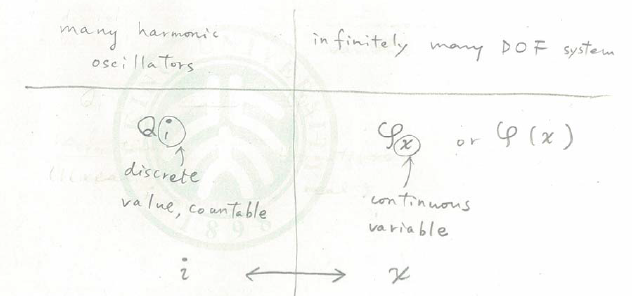
\includegraphics[width = 10cm]{1-1.png}
\end{figure}

An example of the system is a drumhead vibration. Here is a picture of drum:

\begin{figure}[h]
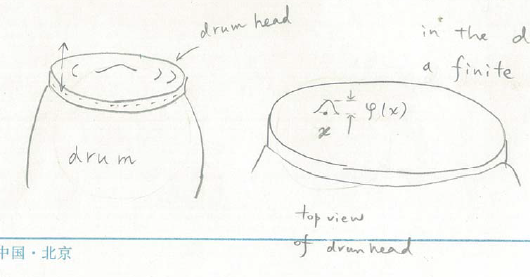
\includegraphics[width = 8cm]{1-2.png}
\end{figure}

Every spatial point in the drumhead can have a finite displacement poerpendicular to the flat drumhead. 

We can define $\varphi$ of $x$ ($\varphi(x)$) as a dispalcement at $x$ point. 

Namely, a given $\varphi$ of $x$ specifies how the drumhead is deformed from the flat drum head. 

Let us consider $\varphi$ of $x$ whose motion is described by the following Lagragian

\begin{align}
L(\varphi,\dot{\varphi}) = \frac{1}{2}\int d^2 x\dot{\varphi}(x)\dot{\varphi}(x) - \frac{1}{2}\int d^2 x \int d^2 x' K(x-x')\varphi(x)\varphi(x')\text{ with }K(x-x') = K(x'-x)
\end{align}

The corresponding equation of motion is

\begin{equation}
0 = \frac{\partial}{\partial t}\frac{\delta L}{\delta \dot{\varphi}(x)} - \frac{\delta\dot{L}}{\delta \varphi(x)} = \ddot{\varphi}(x)+\int d^2 x' K(x-x')\varphi(x')
\end{equation}

When the interaction between fields is spatially local like this

\[K(x-x') = -c^2\Delta^2\delta(x-x'), \]

the equation of motion becomes the usual wave equation

\[\nabla^2\varphi(x) - \frac{1}{c^2}\ddot{\varphi}(x) = 0 \]

\hrule

\ 

If we regard that $\varphi(x)$ is a coordinate variable for each $x$, the conjugate momentu to $\varphi$ is

\[\Pi(x) = \frac{\delta L}{\delta \dot{\varphi}(x)} = \dot{\varphi}(x) \]

The Hamiltonian is then 

\begin{align}
H = \int d^2 x \Pi(x) \dot{\varphi}(x) - L = \frac{1}{2}\int d^2 x \Pi(x)\Pi(x)+\frac{1}{2}\int d^2 x \int d^2 x' K(x-x') \varphi(x)\varphi(x')
\end{align}

To quantize the system, we suppose that $\varphi(x)$ and $\Pi(x)$ are Hermitian operators, which satisfy

\begin{align}
\begin{split}
[\varphi(x),\varphi(x')] &= [\Pi(x),\Pi(x')] = 0\\
[\varphi(x),\Pi(\varphi')] &= i\hbar\delta^2(x-x')
\end{split}
\end{align}

In such a case, it is helpful to express the field in the momentum representation, 

\[\tilde{\varphi}(k) = \int d^2 x\varphi(x)e^{-ikx} \]

\[\tilde{\Pi}(x) = \int d^2 x \Pi(x) e^{-ikx} \]

where the inverse transformation is 

\[\varphi(x) = \int\frac{d^2 k}{(2\pi)^2} \tilde{\varphi}(k)e^{ikx} \]

with

\begin{align}
\int \frac{d^2 k}{(2\pi)^2}e^{-ikx} = \delta^2(x)
\end{align}

Since $\varphi(x)$ and $\Pi(x)$ are hermitian, we have

\[\varphi^\dagger(k) = \varphi(-k) \]

\[\Pi^\dagger(k) = \Pi(-k) \]

The commutation relations are

\begin{align}
\begin{split}
[\tilde{\varphi}(k), \tilde{\varphi}(k')] &= [\tilde{\Pi}(k), \tilde{\Pi}(k')] = 0\\
[\tilde{\varphi}(k),\tilde{\Pi}(k')] &= i\hbar(2\pi)^2\delta^2(k+k')
\end{split}
\end{align}

Now let us introduce 

\[\omega^2(k) = \int d^2x K(x)e^{-ikx} \]

Since $K(x) = K(-x)$, $\omega(k)$ is real and even function in $k$. 

\[\omega^*(k) = \omega(k) = \omega(-k) \]

Let uis again assume that $\omega(k)$ are non-negative for all $k$, so that we replace this by $\omega^2(k)$. 

Rewriting the Hamiltonian in terms of these fields and functions, we obtain

\begin{align}
H = \frac{1}{2}\int\frac{d^2 k}{(2\pi)^2}\left[\tilde{\Pi}(-k)\tilde(k)+\omega^2(k)\tilde{\varphi}(-k)\tilde{\varphi}(k)\right] = \frac{1}{2}\int\frac{d^2 k}{(2\pi)^2}\left[\tilde{\Pi}^\dagger (k)\tilde(k)+\omega^2(k)\tilde{\varphi}^\dagger(k)\tilde{\varphi}(k)\right]
\end{align}

We next define annihilation and creation operators as follows, 

\begin{align}
\begin{split}
a(k) &= \frac{1}{\sqrt{2}}\left[\sqrt{\frac{\omega(k)}{\hbar}}\tilde{\varphi}(k)+\frac{i}{\sqrt{\omega(k)\hbar}}\tilde{\Pi}(k)\right]\\
a^\dagger(k) &= \frac{1}{\sqrt{2}}\left[\sqrt{\frac{\omega(k)}{\hbar}}\tilde{\varphi}(k)-\frac{i}{\sqrt{\omega(k)\hbar}}\tilde{\Pi}(k)\right]
\end{split}
\end{align}

Their commutation relations are calculated as follows, 

\[\begin{split}
[a(k),a(k')] &= \frac{1}{2\hbar}\left[\sqrt{\omega_k}\tilde{\varphi}(k)+\frac{i}{\sqrt{\omega_k}} \tilde{\Pi}(k), \sqrt{\omega_{k'}}\tilde{\varphi}(k')+\frac{i}{\sqrt{\omega_{k'}}}\tilde{\Pi}(k')\right] \\
&= \frac{1}{2\hbar}\sqrt{\frac{\omega_k}{\omega_{k'}}}i[\tilde{\varphi}(k),\tilde{\Pi}(k')] + \frac{1}{2\hbar}\sqrt{\frac{\omega_{k'}}{\omega_k}}i[\tilde{\Pi}(k),\tilde{\varphi}(k')] \\
&=(-1)(2\pi)^2\delta^2(k+k')+(2\pi)^2\delta^2(k+k')= 0 
\end{split}\]

\[[a^\dagger(k),a^\dagger(k')] = 0 \]

\begin{align}\begin{split}
[a(k),a^\dagger(k')] &= \frac{1}{2\hbar}\left[\sqrt{\omega_k}\tilde{\varphi}(k)+\frac{i}{\sqrt{\omega_k}}, \sqrt{\omega_{k'}}\tilde{\varphi}(-k') - \frac{i}{\sqrt{\omega_{k'}}}\tilde{\Pi}(-k')\right] \\
&= \frac{-i}{2\hbar}\sqrt{\frac{\omega_k}{\omega_{k'}}} [\tilde{\varphi}(k),\tilde{\Pi}(-k')] + \frac{i}{2\hbar}[\tilde{\Pi}(k),\tilde{\varphi}(-k')] \\
&= (2\pi)^2\delta^2(k-k')
\end{split}\end{align}

If we wrtie $H$ in terms of $a \& a^\dagger$, we obtain

\begin{align}
H = \frac{1}{2}\int \frac{d^2 k}{(2\pi)^2}\hbar\omega(k)[a^\dagger(k)a(k)+a(k)a^\dagger(k)] = \frac{1}{2}\int \frac{d^2 k}{(2\pi)^2}\hbar\omega(k)a^\dagger(k)a(k)+C
\end{align}

Thus, eigenstate of $H$ is given by the repeated application of $a^\dagger(k)$ onto the ground state\footnote{Regarding these energy units as particles respectively, we can think of these excited states as one-particle state, two-particle state, and so on. }

\[|k_1\rangle = a^\dagger(k_1)|0\rangle,\quad (E=\omega(k_1)) \]
\[|k_1,k_2\rangle = a^\dagger(k_1)a^\dagger(k_2)|0\rangle,\quad (E=\omega(k_1)+\omega(k_2)) \]

while the ground state satisfies

\[a(k)|0\rangle = 0,\quad\text{for}\forall k \]

To characterize these multi-particle states, let us consider the following operators, 

\begin{align}
\mathbb{P} \equiv\int\frac{d^2 k}{(2\pi)^2}\hbar{k}a^\dagger({k})a({k})
\end{align}

which satisfies

\[[\mathbb{P},a^\dagger({k})] = \hbar {k}a^\dagger(k) \]
\[[\mathbb{P},a(k)] = -\hbar ka(k) \]

so that

\[\begin{split}
\mathbb{P}|k_1,k_2,\cdots\rangle &= \mathbb{P}a^\dagger(k_1)a^\dagger(k_2)\cdots|0\rangle  = a^\dagger(k_1)(\hbar k_1+\mathbb{P})a^\dagger(k_2)\cdots|0\rangle\\
&= \hbar k_1 |k_1,k_2,\cdots\rangle + a^\dagger(k_1)\mathbb{P}a^\dagger(k_2)\cdots|0\rangle\\
&= \hbar k_1|k_1,k_2,\cdots\rangle + a^\dagger(k_1)a^\dagger(k_2)(\hbar k_2+\mathbb{P})\cdots|0\rangle\\
&=\cdots\\
&=\hbar(k_1+k_2+\cdots)|k_1,k_2,\cdots\rangle
\end{split}\]

we can also see that

\[\begin{split}
[\mathbb{P},\varphi(x)] &= \left[\mathbb{P},\int\frac{d^2k}{(2\pi)^2}\sqrt{\frac{\hbar}{2\omega(k)}}\left(a(k)e^{ik\cdot x}+a^\dagger(k)e^{-ik\cdot x}\right)\right]\\
&= \int\frac{d^2 k}{(2\pi)^2}\sqrt{\frac{\hbar}{2\omega(k)}}\left\{(-\hbar k)a(k)e^{ik\cdot x}+(\hbar k)a^\dagger(k)e^{-ik\cdot x}\right\}\\
&= i\hbar\frac{\partial}{\partial x}\left\{\int\frac{d^2 k}{(2\pi)^2}\sqrt{\frac{\hbar}{2\omega(k)}}\left(a(k)e^{ik\cdot x}+a^\dagger(k)e^{-ik\cdot x}\right)\right\}\\
&=i\hbar\frac{\partial}{\partial x}\varphi(x)
\end{split}\]

Similarly

\[[\mathbb{P},\Pi(x)] = i\hbar\cdot\frac{\partial}{\partial x}\Pi(x) \]

Using these relations, one can show that 

\[e^{a\cdot\mathbb{P}/i\hbar}\varphi(x)e^{-a\cdot\mathbb{P}/i\hbar} = \varphi(x+a) \]
\[e^{a\cdot\mathbb{P}/i\hbar}\Pi(x)e^{-a\cdot\mathbb{P}/i\hbar} = \Pi(x+a) \]

Namely, taking a derivative of r.h.s with respect to $a$, we have

\[\begin{split}
\frac{\partial}{\partial a}\left[e^{a\cdot\mathbb{P}/i\hbar}\varphi(x)e^{-a\cdot\mathbb{P}/i\hbar}\right]&=\frac{1}{i\hbar}e^{a\cdot\mathbb{P}/i\hbar}[\mathbb{P},\varphi(x)]e^{-a\cdot\mathbb{P}/i\hbar}\\
&= e^{a\cdot\mathbb{P}/i\hbar}\frac{\partial}{\partial x}\varphi(x)e^{-a\cdot\mathbb{P}/i\hbar}\\
&=\frac{\partial}{\partial x}\left\{e^{a\cdot\mathbb{P}/i\hbar}\varphi(x)e^{-a\cdot\mathbb{P}/i\hbar}\right\}
\end{split}\]

This means that

\[e^{a\cdot\mathbb{P}/i\hbar}\varphi(x)e^{-a\cdot\mathbb{P}/i\hbar} = f(x+a) \]

while $f$ should be $\phi$ when $a=0$, thus we have

\begin{align}
e^{a\cdot\mathbb{P}/i\hbar}\varphi(x)e^{-a\cdot\mathbb{P}/i\hbar} = \varphi(x+a)
\end{align}

Similar we have

\[e^{a\cdot\mathbb{P}/i\hbar}\Pi(x)e^{-a\cdot\mathbb{P}/i\hbar} = \Pi(x+a)
\]

These two relations means that $\mathbb{P}$ is a generator of the spatial translation and is therefore the momentum operator. 


\section{System of indistinguishable particles}

In the preceding sections, we consider the quantum states of an oscillator  system as multiparticle states, where each particle has an energy unit and is often called a ``phonon''. In this section, we follow a different line of reasoning. We will start with a space of states describing a single particle, which is either Bose particle or Fermi particle. We then construct the multiple-particle states based on standard methods. 

For the Bose particle case, we will arrive at a system of states and operators, that is mathematically equivalent to that found previously for a systen of oscillators. Thereby, this shows that the interpretation of oscillator states as many-phonon states is consistent with the usual description of many-particle systems with Bose statistics. 

We will develop a formalism with Fermi-Dirac statistics, for which the states do not resemble those of a harmonic-oscillator system. 

Consider first the case of distinguishable particles. 

A $n$-particle state is given by a simple product of one-particle states

\[|\psi\rangle = |\psi_1\rangle|\psi_2\rangle\cdots|\psi_n\rangle \]

You can also weite this in the coordinate representation as 

\[\psi(x_1,\cdots,x_n) = \psi_1(x_1)\psi_2(x_2)\cdots\psi_n(x_n) \]

where $x_j$ denotes the coordinate of $j$-th particle and $\langle x_j|\psi_j\rangle = \psi_j(x_j)$. 

Please notice that these $n$-particles are all distinguishable from one another. 

Namely, each particle has its own coordinate $x$, and we can distinguish $j$-th particle from $m$-th particle, because they belong to different one-particle states

\[\psi_j(x) \neq \psi_m(x),\quad \text{for }j\neq m \]

\hrule

\ 

Let us next consider indistinguishable particles. 

To make up a many-particle wavefunction for indistinguishable particles out of this, we need to make any pair of particles cannot be distinguished from each other. 

There is two-ways of doing this, one way is to ``symmetrize'' this with respect to all the possible permutations of $n$ particles:

\[\psi_1(x_1)\cdot\psi_2(x_2)\cdot\cdots\cdot\psi_n(x_n)\overset{\text{``symmetrize''}}{\longrightarrow}\frac{1}{\sqrt{n!}}\sum_P \psi_{P(1)}(x_1)\cdot\psi_{P(2)}(x_2)\cdot\cdots\cdot\psi_{P(n)}(x_n) \]

Here $P$ denotes a permutation among $n$ numbers, $\{1,2,\cdots,n\}$

\[P \equiv\left(
\begin{matrix}
1 & 2 & \cdots & n\\
P(1) & P(2) & \cdots & P(n)
\end{matrix}
\right) \]

into $\{P(1),P(2),\cdots P(n)\}$

we take the sum over all possible permutations here. 

The total number of possible permutations among $n$ distinguishable objects are given by a factorial of $n$. To normalize this many-particle wavefunction, I put $1$ over the square root of the factorial of $n$. We can see that the exchange between the $j$-th particle coordinate and the $m$-th particle coordinate does not change this many-particle wavefunction. 

\[\begin{split}
\psi(x_2,x_1,x_3,\cdots x_n) &= \frac{1}{\sqrt{n!}}\sum_P\psi_{P(1)}(x_2)\psi_{P(1)}(x_2)\psi_{P(3)}(x_3)\cdots\psi_{(P(n)}(x_n)\\
&=\frac{1}{\sqrt{n}}\sum_P\psi_{P(1)}(x_2)\psi_{P(1)}(x_2)\psi_{P(3)}(x_3)\cdots\psi_{(P(n)}(x_n)\\
\Big\{P' &= P\cdot\left(
\begin{matrix}
1 & 2 & 3 & \cdots & n\\
2 & 1 & 3 & \cdots & n
\end{matrix}\right)\Big\}\\
&=\frac{1}{\sqrt{n}}\sum_{P'}\psi_{P'(1)}(x_1)\psi_{P'(2)}(x_2)\psi_{P'(3)}(x_3)\cdots\psi_{P'(n)}(x_n)\\
&= \psi(x_1,x_2,x_3,\cdots, x_n)
\end{split}\]

Here $P'$ is a product between a permutation $P$ and the permutation which exchange $1$ and $2$, while remains other indices intact. 

This product can be regarded as a mapping from $P$ to $P'$ and this mapping is one-to-one mapping. 

Namely, a set of all possible permutations is unchanged under that mapping. 

Therefore, the right hand side is identical to the original wavefunctions. 

This argument so far holds true not only for the exchange between arbitrary pair of two particles but also for an arbitrary permutations among $n$ particles. 

\[\psi(x_{Q(1)},x_{Q(2)},\cdots,x_{Q(n)}) = \cdots=\psi(x_1,x_2,\cdots,x_n) \]

Because of this symmetrized property, $n$-particles in this wavefunction are indistinguishable from one another. 

An indistinguishable particle in a symmetrized many-particle wavefunction is called as ``boson''. 

The other way of making wavefunctions for indistinguishable particles is ``antesymmetrize'' the wavefunction for distinguishable particles. %page41

\[\Psi_F(x_1,\cdots,x_n) = \frac{1}{\sqrt{n!}}\sum_P(-1)^P\psi_{P(1)}(x_1)\cdot\psi_{P(2)}(x_2)\cdot\cdots\cdot\psi_{P(n)}(x_n) \]

Here $P$ us again in a permutation among $n$-particles, but, at this time, we have $(-1)^P$ ($(-1)$ to the power of $P$). This factor takes $+1$, if the permutation $P$ is given by a product of even-number of transpositions, where a transposition is an exchange between a pair of two particle. 

For example, 

\[
\left(\begin{matrix}
1 & 2 & 3\\ 2 & 3 & 1
\end{matrix}\right) = 
\left(\begin{matrix}
1 & 2 & 3\\ 2 & 1 & 3
\end{matrix}\right)
\cdot
\left(\begin{matrix}
1 & 2 & 3\\ 1 & 3 & 2
\end{matrix}\right)
\]

\[((1,2,3)\rightarrow(2,1,3)\rightarrow(2,3,1) \]

this permutation is given by a product of two transpositions, so that

\[(-1)^{\left(\begin{matrix}
1 & 2 & 3\\ 2 & 3 & 1
\end{matrix}\right)} = +1 \]

This factor takes $-1$, if the permutation $p$ is given by a product of odd-numbers of transpositions. 

For example, 

\[
\left(\begin{matrix}
1 & 2 & 3 & 4\\ 2 & 3 & 4 & 1
\end{matrix}\right)=
\left(\begin{matrix}
1 & 2 & 3 & 4\\ 2 & 1 & 3 & 4
\end{matrix}\right)
\cdot
\left(\begin{matrix}
1 & 2 & 3 & 4\\ 1 & 3 & 2 & 4
\end{matrix}\right)
\cdot
\left(\begin{matrix}
1 & 2 & 3 & 4\\ 1 & 2 & 4 & 3
\end{matrix}\right)
\]

this permutation is given by a product of three transpositions, so that 

\[(-1)^{\left(\begin{matrix}
1 & 2 & 3 & 4\\ 2 & 3 & 4 & 1
\end{matrix}\right)}  = -1\]

Under a permutation among $n$ particles, this many-body wavefunction is unchanged, apart from the phase factor, which is $(-1)$ to the power of $Q$. 

 \[\begin{split}
&\psi_F(x_{Q(1)},x_{Q(2)},\cdots,x_{Q(m)}) \\
&=\frac{1}{\sqrt{n!}}\sum_P(-1)^P\psi_{P(1)}(x_{Q(1)})\cdot\cdots\cdot\psi_{P(n)}(x_{Q(n)})\\
&=\frac{1}{\sqrt{n!}}\sum_P(-1)^P\psi_{P\cdot Q^{-1}(1)}(x_1)\cdot\cdots\cdot\psi_{P\cdot Q^{-1}(n)}(x_n)\\
&\quad\quad P\cdot Q^{-1}=1\\
&=(-1)^Q\frac{1}{\sqrt{n!}}\sum_{P'}(-1)^{P'}]psi_{P'(1)}(x_1)\cdot\cdots\cdot\psi_{P'(n)}(x_n)\\
&=(-1)^Q\psi_F(x_1,\cdots,x_n)
\end{split}\]

Because of this, asymmetrized property, $n$-particle in the wavefunction are essentially indistinguishable from one another. 

An indistinguishable particle in an antisymmetrized many-particle wavefunction is called as ``fermion''. 

To summarize so far, we have two way of making many-particle wavefunctions for indistinguishable particles. 

\begin{align}
|\psi\rangle &= \frac{1}{\sqrt{n!}}\sum_P\xi^P|\psi_{P(1)}\rangle|\psi_{P(2)}\rangle\cdots|\psi_{P(n)}\rangle\\
\psi(x_1,\cdots,x_n) &= \frac{1}{\sqrt{n!}}\sum_P\xi^P\psi_{P(1)}(x_1)\psi_{P(2)}(x_2)\cdot\cdots\cdot\psi_{P(n)}(x_n) = \frac{1}{\sqrt{n!}}\sum_P\xi^P\psi_1(x_{P(1)})\psi_2(x_{P(2)})\cdot\cdots\cdot\psi_n(x_{P(n)}) \end{align}

where $\xi = \pm1$ for boson and fermion. 

We will write this as $|\psi_1,\psi_2,\psi_n,\cdots\psi_n\rangle$. 

Let us show an example:

Suppose that $|\psi_1\rangle$ and $|\psi_2\rangle$ are two orthonormal single-particle states. 

For bose particles, we can make three many-particle wavefunctions out of them. One is this, and the other is

\[\begin{split}
|\Psi_a\rangle &= \frac{1}{\sqrt{2!}}(|\psi_1\rangle|\psi_2\rangle + |\psi_2\rangle|\psi_1\rangle)\\
|\Psi_b\rangle &= \frac{1}{\sqrt{2!}}(|\psi_1\rangle|\psi_1\rangle + |\psi_1\rangle|\psi_1\rangle) = \sqrt{2}|\psi_1\rangle|\psi_1\rangle\\
|\Psi_c\rangle &= \frac{1}{\sqrt{2!}}(\psi_2\rangle|\psi_2\rangle + \psi_2\rangle|\psi_2\rangle) = \sqrt{2}\psi_2\rangle|\psi_2\rangle
\end{split} \]

For fermi particles, we can make only one many-particle wavefunctions, 

\[\begin{split}
|\Psi_a\rangle &= \frac{1}{\sqrt{2!}}(|\psi_1\rangle|\psi_2\rangle - |\psi_2\rangle|\psi_1\rangle) \\
|\Psi_b\rangle &= \frac{1}{\sqrt{2!}}(|\psi_1\rangle|\psi_1\rangle - |\psi_1\rangle|\psi_1\rangle) = 0 \\
|\Psi_b\rangle &= \frac{1}{\sqrt{2!}}(|\psi_2\rangle|\psi_2\rangle - |\psi_2\rangle|\psi_2\rangle) = 0 
\end{split}\] 

This two dictates that, due to the antisymmetric character, two fermi particles cannot occupy the same state. 

The inner product of two of these $n$-particle states are given by a determinent or permanent of a $n\times n$ matrix, which is composed by the inner products of single particle states. 

\begin{align}
\langle\varphi_1,\cdots,\varphi_n|\psi_1,\cdots,\psi_n\rangle = \begin{vmatrix}
\langle \varphi_1|\psi_1\rangle & \langle \varphi_1|\psi_2\rangle & \cdots & \langle \varphi_1|\psi_n\rangle\\
\langle \varphi_2|\psi_1\rangle & \langle \varphi_2|\psi_2\rangle & \cdots & \langle \varphi_2|\psi_n\rangle\\
\cdots & \cdots & \cdots & \cdots\\
\langle \varphi_n|\psi_1\rangle & \langle \varphi_n|\psi_2\rangle & \cdots & \langle \varphi_n|\psi_n\rangle
\end{vmatrix}
\end{align}

where 

\[\langle\varphi_j|\psi_m\rangle = \int d^d {\bf x}\varphi_j^*({\bf x})\psi_m({\bf x}) \]

and

\[|{\bf A}|_{\xi} = \sum_{P}\xi^P {\bf A}_{1P(1)}\cdots{\bf A}_{nP(n)} \]

with $n\times n$ matrix ${\bf A} = ({\bf A}_{ij})$

Namely, $|{\bf A}|$ is a determinant of ${\bf A}$ while ${\bf A}_+$ is a permanent of ${\bf A}$. 

\hrule

\ 

One can prove this straightforwardly, 

\[\begin{split}
&\langle\varphi_1,\cdots,\varphi_n|\psi_1,\cdots,\psi_n\rangle =\frac{1}{n!}\sum_P\sum_Q\xi^P\xi^Q\langle\varphi_{P(1)}|\psi_{Q(1)}\rangle\cdots\langle\varphi_{P(n)}|\psi_{Q(n)}\rangle \\
& = \frac{1}{n!}\sum_{P}\sum_{Q}\xi^P\xi^Q\langle\varphi_1|\psi_{QP^{-1}(1)}\rangle\cdots\langle\varphi_n|\psi_{QP^{-1}(n)}\rangle\\
&\quad (\xi^P)^{-1} = \xi^P,\quad R\equiv Q\cdot P^{-1}\\
&= \frac{1}{n!} \sum_P\sum_Q\xi^R\langle\varphi_1|\psi_{R(1)}\rangle\cdots\langle\varphi_n|\psi_{R(n)}\rangle
\end{split}\]

\[\sum_P\sum_Q = \sum_P\sum_{QP^{-1}}=\sum_P\sum_R \]

Now that the summation is free from $P$, the summation over $P$ just gives us a factor $n!$, which set off this. 

Thus, we have

\[\langle\varphi_1,\cdots,\varphi_n|\psi_1,\cdots,\psi_n\rangle = \sum_R\xi^R\langle\varphi_1|\psi_{R(1)}\rangle\cdots\langle\varphi_n|\psi_{R(n)}\rangle = |(\langle\varphi_i|\psi_j\rangle)|_\xi \]

Suppose that $\{|1\rangle,|2\rangle,\cdots\}$ is a complete orthonormal set of single-particle states:

\[\alpha|\beta\rangle = \delta_{\alpha\beta},\quad\sum_{\alpha}|\alpha\rangle\langle\alpha| = 1 \]

A complete set of $n$-particle states consists of $|\alpha_1,\alpha_2,\cdots,\alpha_n\rangle$ where $\alpha_1\le\cdots\le\alpha_n$ in the Bose case, and $\alpha_1<\alpha_2<\cdots<\alpha_n$ in the fermion case. 

These states are orthogonal to one another, but not always normalized in the Bose case. 

Using this, one can show that a complete orthonormal set of $n$-particle states consist of

\begin{align}\begin{cases}
\displaystyle\frac{|\alpha_1,\alpha_2,\cdots,\alpha_n\rangle}{\sqrt{n_1!n_2!\cdots}} \quad (\alpha_1\le\cdots\le\alpha_n) \ \text{for boson}\\
\ \\
|\alpha_1,\alpha_2,\cdots\alpha_n\rangle \quad (\alpha_1<\alpha_2<\cdots<\alpha_n)\ \text(for fermion)
\end{cases}\end{align}

where $n_j$ denotes the number of times that $j$ occurs in the sequence of $\alpha_1,\cdots,\alpha_n$. 

For either boson case or fermion case, the completeness relation in the $n$-particles space can be weitten in the following simple form. 

\begin{align}
\frac{1}{n!}\sum_{\alpha_1}\cdots\sum_{\alpha_n}|\alpha_1,\cdots,\alpha_n\rangle\langle\alpha)_1,\cdots,\alpha_n| = 1
\end{align}

where the sum of each $\alpha_j$ is taken over all single-particle states. 

The duplication of $n$-particle states are set off by the $1/n!$ (one over the factorial of $n$) and the normalization. 

To see that this equality holds true for both boson and fermion cases, let us apply the left side to a $n$-particle state $|\beta_1,\cdots,\beta_n\rangle$ where $|\beta_j\rangle$ is from $\{|1\rangle,|2\rangle,\cdots,\}$ the single-particle states considered. \\

{\Huge 1. }When all these $\beta_j$ are distict from one another, 

\[\begin{split}
&\frac{1}{n!}\sum_{\alpha_1}\cdots\sum_{\alpha_n}|\alpha_1,\cdots,\alpha_n\rangle\langle\alpha_1,\cdots,\alpha_n|\beta_1,\cdots,\beta_n\rangle\\
&=\frac{1}{n!}\sum_P|P(\beta_1),P(\beta_2),\cdots,P(\beta_n)\rangle\langle P(\beta_1),P(\beta_2),\cdots,P(\beta_n)|\beta_1,\cdots,\beta_n\rangle\\
&=\frac{1}{n!}\sum_P\xi^P|P(\beta_1),P(\beta_2),\cdots,P(\beta_n)\rangle\\
&=\frac{1}{n!}\sum_P|\beta_1,\cdots,\beta_n\rangle = |\beta_1,\cdots,\beta_n\rangle
\end{split}\]

{\Huge 2. }When some of these $\beta_j$ are identical, which can be the case with bose particles, 

\[\begin{split}
&\frac{1}{n!}\sum_{\alpha_1}\cdots\sum_{\alpha_n}|\alpha_1,\cdots,\alpha_n\rangle\langle\alpha_1,\cdots,\alpha_n|\beta_1,\cdots,\beta_n\rangle \\
&= \frac{1}{n!}{\color{red}{\tilde{\sum_P}}}|P(\beta_1),P(\beta_2),\cdots,P(\beta_n)\rangle\langle P(\beta_1),P(\beta_2),\cdots,P(\beta_n)|\beta_1,\cdots,\beta_n\rangle \end{split}\]

Here the {\color{red}{summation}} of $P$ is taken over all possible permutations of $n$-objects with duplications being excluded. 

Namely, $\tilde{\sum_P}$ does count the following permutations separately. It counts one of them once and doesn't count the others. 

\[
\begin{split}
&P_1(\beta_j) = P_2(\beta_j) = P_3(\beta_j)=\cdots=P_m(\beta_j), \text{ for }\forall j = 1,\cdots,n\\ 
&=\frac{1}{n!}\tilde{\sum_P}|P(\beta_1),\cdots,P(\beta_n)\rangle\times(n_1!\cdot n_2!\cdots)
\end{split}\]

where $n_j$ denotes the number of times that ``$j$'' occurs in the sequence of $\beta_1,\cdots,\beta_n$. 

Now that 

\[|P(\beta_1),\cdots,P(\beta_n)\rangle = |\beta_1,\cdots,\beta_n\rangle \]

and

\[\tilde{\sum_P} = \frac{n!}{n_1!\cdot n_2!\cdot\cdots} \]

the right hand side is

\[=|\beta_1,\beta_2,\cdots,\beta_n\rangle \]

\ 

These two ({\Huge 1, 2}) prove that this completeness relation holds true for both boson case and fermion case. \\

\hrule

\ 

In actual physical process, the number of particles is not constant in time. Particles can be constructed and destroyed. To describe such process, we need a Hilbert space that contains states of varying number of particles. To get such a space, we simply combine all the $n$-particle spaces into one big space that we call the ``multiparticle space''. 

A general state in the multiparticle space is of the from of 

\[|\psi\rangle = |\psi^{(0)}\rangle + |\psi^{(1)}\rangle + |\psi^{(2)}\rangle + \cdots \]

where $|\psi^{(n)}\rangle$ is an $n$-particle state and $|\psi^{(0)}\rangle$ is just a vacuum state

\[|\psi^{(0)}\rangle = |var\rangle \]

States of differemt numbers of particles are defined to be orthogonal to each other, so that

\[\langle\varphi|\psi\rangle = \langle\varphi^{(0)}|\psi^{(0)}\rangle + \langle\varphi^{(1)}|\psi^{(1)}\rangle  \]

where

\[|\varphi\rangle = |\varphi^{(0)}\rangle + |\varphi^{(1)}\rangle + \cdots \]

The completeness relation in the multiparticle is given as follows, 

\begin{align}
\sum_{n=1}^{\infty}\frac{1}{n!}\sum_{\alpha_1}\cdots\sum_{\alpha_n}|\alpha_1,\cdots,\alpha_n\rangle\langle \alpha_1,\cdots,\alpha_n| = 1
\end{align}



\section{Creation operator \& destruction operator}

So far, we have constructed a complete orthonormal set of states in the multiparticle space. With these constructions in hand, we are now ready to define creation and destruction operators. These operators change the number of particles, so that they connect states of different numbers of particles. We will see that allthe physical operators are expressed in terms of creation and destruction operators. 

Let $|\varphi\rangle$ be any one-particle state. We define $a^\dagger$ of $\varphi$ to be that linear operator which satisfies this, for any n-particle states $|\psi_1, \cdots,\psi_n\rangle$. 

\begin{align}
a^\dagger{\varphi}|\psi_1,\cdots,\psi_n\rangle = |\varphi,\psi_1,\cdots,\psi_n\rangle \tag{e}\\
\quad\text{for any}|\psi_1,\cdots,\psi_n\rangle \label{Eqs1.6.1}
\end{align}

For $n=0$, this simply means that

\[a^\dagger(\varphi)|vac\rangle = |\varphi\rangle \]

We call $a^\dagger(\varphi)$ as the creation operator for the state $|\varphi\rangle$, and its hermitian conjugate $a(\varphi)$ as the destruction or annihilation operator. 

A destruction operator converts an $n$-particle states into a $(n-1)$-particle states. 

To find the effect of $a(\varphi)$ on an $n$-particle state $|\psi_1,\psi_2,\cdots,\psi_n\rangle$, we multiply on the left by an arbitrary $(n-1)$-particle state, which is this

\[\begin{split}
&\langle x_1,\cdots,x_{n-1}|a(\varphi)|\psi_1,\cdots,\psi_n\rangle \\
&= (\langle \psi_1,\cdots,\psi_n|a^\dagger(\varphi)|x_1,\cdots,x_{n-1}\rangle)^*\\
&= (\langle \psi_1,\cdots,\psi_n|\varphi,x_1,\cdots,x_{n-1}\rangle)^*\\
&= 
\begin{vmatrix}
\langle\psi_1|\phi\rangle & \langle\psi_1|x_1\rangle & \cdots & \langle\psi_1|x_{n-1}\rangle\\
\langle\psi_2|\phi\rangle & \langle\psi_2|x_1\rangle & \cdots & \langle\psi_2|x_{n-1}\rangle\\
\cdots & \cdots & \cdots & \cdots \\
\langle\psi_n|\phi\rangle & \langle\psi_n|x_1\rangle & \cdots & \langle\psi_n|x_{n-1}\rangle
\end{vmatrix}_{\xi}^*\\
&= \left\{\sum_{k=1}^n \xi^{k-1}\langle\psi_k|\varphi\rangle
\begin{vmatrix}
 \langle\psi_1|x_1\rangle & \cdots & \langle\psi_1|x_{n-1}\rangle\\
 \langle\psi_2|x_1\rangle & \cdots & \langle\psi_2|x_{n-1}\rangle\\
 \cdots & \cdots & \cdots \\
 \langle\psi_n|x_1\rangle & \cdots & \langle\psi_n|x_{n-1}\rangle
\end{vmatrix}_{\xi} \right\}^*\\
&= \sum_{k=1}^n \xi^{k-1}\langle\varphi|\psi_k\rangle\langle x_1,\cdots,x_{n-1}|\psi_1,\cdots,\psi_{k-1},\psi_{k+1},\cdots,\psi_n\rangle
\end{split}\]

Since this relation holds true for any arbitrary $x_1$ and so on, we finally have

\begin{align}\label{Eqs1.6.2}a(\varphi)|\psi_1,\cdots,\psi_n\rangle = \sum_{k=1}^n \xi^{k-1}\langle \varphi|\psi_k\rangle |\psi_1,\cdots,\psi_{k-1},\psi_{k+1},\cdots,\psi_n\rangle \end{align}


We can derive 

\[a^\dagger(\varphi_1)a^\dagger(\varphi_2) = \xi a^\dagger(\varphi_2)a^\dagger(\varphi) \]

Namely, the following relations holds true for arbitrary $\psi_1,\cdots,\psi_n$

\[a^\dagger(\varphi_1)a^\dagger(\varphi_2)|\psi_1,\cdots,\psi_n\rangle = \xi a^\dagger(\varphi_2)a^\dagger(\varphi) |\psi_1,\cdots,\psi_n\rangle\]

This leads to the commutation relations for boson and fermion. 

\begin{align}
[a^\dagger(\varphi_1),a^\dagger(\varphi_2)]_{-\xi} = 0
\end{align}

where

\[[A,B]_{-\xi} = AB - \xi BA = \begin{cases}AB-BA\ \text{boson}\\ \ \\ AB+BA \ \text{fermion}\end{cases}\]

Taking the hermite conjugate of this, we have

\begin{align}
[a(\varphi_1),a(\varphi_2)]_{-\xi} = 0
\end{align}

\hrule

\ 

To find the commutation relations between the creation operator and destruction operator, we first calculate 

\[\begin{split}
&a(\varphi_1)a^\dagger(\varphi_2)|\psi_1,\cdots,\psi_n\rangle \\
&=a(\varphi_1)|\varphi_2,\psi_1,\cdots,\psi_n\rangle\\
&= \langle\varphi_1|\varphi_2\rangle|\psi_1,\cdots,\psi_n\rangle + \sum_{k=1}^n\xi^k\langle\varphi_1|\psi_k\rangle|\varphi_2,\psi_1,\cdots,\psi_{k-1},\psi_{k+1},\cdots,\psi_n\rangle
\end{split}\]

and

\[\begin{split}
&a^\dagger(\varphi_2)a(\varphi_1)|\psi_1,\cdots,\psi_n\rangle \\
&= \sum_{k=1}^n\xi^{k-1}\langle \varphi_1|\psi_k\rangle a^\dagger(\varphi_2)|\psi_k\rangle|\varphi_2,\psi_1,\cdots,\psi_{k-1},\psi_{k+1},\cdots,\psi_n\rangle\\
&= \sum_{k=1}^n\xi^{k-1}\langle \varphi_1|\psi_k\rangle |\varphi_2,\psi_k\rangle|\varphi_2,\psi_1,\cdots,\psi_{k-1},\psi_{k+1},\cdots,\psi_n\rangle\\
\end{split}\]

Multiply this by $\xi$ and substract it from the former one, we see that

\[[a(\varphi_1)a^\dagger(\varphi_2) - \xi a^\dagger(\varphi_2)a(\varphi_2)]|\psi_1,\cdots,\psi_n\rangle = \langle \varphi_1|\varphi_2\rangle |\psi_1,\cdots,\psi_n\rangle \]

Equivalently, we have

\begin{align}\label{eqs1.6.5}
[a(\varphi_1),a^\dagger(\varphi_2)] _{-\xi} = \langle\varphi_1|\varphi_2\rangle
\end{align}

These three relations are the fundamental ``commutation relations'' for creation \& destruction operators. When these operators are introduced in terms of an orthonormal basis, this relation becomes

\begin{align}
[a(\alpha),a^\dagger(\beta)]_{-\xi} = \langle\alpha|\beta\rangle = \delta_{\alpha\beta}
\end{align}

Where one-particle states $|\alpha\rangle$ and $|\beta\rangle$ are from a complete orthonormal set of one-particle states, $\{|1\rangle,|2\rangle,\cdots\}$

Let us next compare these commutation relations with raising and lowering operators for linear harmonic osciallators. 

For boson case, we further define an orthonormal basis for the multiparticle space as 

\begin{align}|n_1,n_2,\cdots\rangle = \frac{|\overset{n_1}{1,\cdots,1},\overset{n_2}{2,\cdots,2},\cdots\rangle}{\sqrt{n_1! n_2!,\cdots}} \end{align}

Where we use $\{|1\rangle,|2\rangle,\cdots\}$ as a complete orthonormal set of one-particle states and $n_{\alpha}$ is the number of times $\alpha$ appear in the ket state in the right hand side. In terms of this orthornormal basis, eqs \eqref{Eqs1.6.1}, \eqref{Eqs1.6.2} reduce to the followings:

\begin{align}
a^\dagger(\alpha)|n_1,n_2,\cdots,n_{\alpha},\cdots\rangle = \sqrt{n_\alpha+1}|n_1,n_2,\cdots,n_{\alpha}+1,\cdots\rangle\\
a(\alpha)|n_1,n_2,\cdots,n_{\alpha},\cdots\rangle = \sqrt{n_\alpha}|n_1,n_2,\cdots,n_{\alpha}-1,\cdots\rangle
\end{align}

while the commutation relations are 

\begin{equation}
\begin{split}
[a(\alpha),a(\beta)] &= [a^\dagger(\alpha),a^\dagger(\beta)] = 0\\
[a(\alpha),a^\dagger(\beta)] &= \delta_{\alpha\beta}
\end{split}
\end{equation}

These three equations are identical to eqs \eqref{Eqs1.3.2}, \eqref{Eqs1.3.3}, \eqref{Eqs1.3.4}

This means that creation \& destruction operators for a system of Bose particles looks exactly like those for a system of linear harmonic oscillators. 

For fermions case, we have

\begin{align}
\begin{split}
a_\alpha^\dagger|\alpha_1,\cdots,\alpha_n\rangle &= |\alpha,\alpha_1,\cdots,\alpha_n\rangle\\
a_\alpha|\alpha_1,\cdots,\alpha_n\rangle &= \sum_{k=1}^n(-1)^{k-1}\delta_{\alpha\alpha_k}|\alpha_1,\cdots,\alpha_{k-1},\alpha_{k+1},\cdots,\alpha_n\rangle
\end{split}
\end{align}

\begin{align}
\begin{cases}
[a_\alpha,a_\beta]_+ = [a_\alpha^\dagger,a_\beta^\dagger] = 0\\
[a_\alpha,a_\beta^\dagger]_+ = \delta_{\alpha\beta}
\end{cases}
\end{align}

Contrary to the boson case, there is no a priori reason for  postulating these anticommutation relations. These relations can be derived only from the antisymmetrization postulate for fermions. 

Let us put some remarks on these general commutation relations. 

One advantage of deriving them in such a general form is that we are not tied down to a particular basis of one-particle states. Suppose we use a basis of momentum eigenstates, $|\bf p\rangle$ with $\langle{\bf p}|{\bf p'}\rangle = (2\pi)^3\delta^3({\bf p}-{\bf p'})$. Then we have

\begin{align}
\begin{split}
[a({\bf p}),a^\dagger({\bf p'})]_{-\xi}&=(2\pi)^3\delta^3({\bf p}-{\bf p'})\\
[a({\bf p}), a({\bf p'})]_{-\xi} &= [a^\dagger({\bf p}),a^\dagger({\bf p'})]_{-\xi} = 0
\end{split}
\end{align}

A complete orthogonal sets of states in the multiparticle space can be constructed from the vacuum state 

\[|{\bf p_1},{\bf p_2},\cdots,{\bf p_n}\rangle = a^\dagger({\bf p_1})\cdots a^\dagger({\bf p_n})|vac\rangle \]

If we use a basis of position eigenstates $|\bf{x}\rangle$ with $\langle {\bf x}|{\bf x'}\rangle = \delta^3({\bf x} - {\bf x'})$

\begin{align}
[a({\bf x}),a^\dagger({\bf x'})] = \delta^3({\bf x} - {\bf x'})
\end{align}

\[|{\bf x}_1,\cdots,{\bf x}_n\rangle = a^\dagger({\bf x}_1)\cdots a^\dagger({\bf x}_n)|vac\rangle \]

When we change a basis for one-particle states, the creation operators ``transform'' like ket state, while the destruction operators ``transform'' like bra state. 

\[|{\bf x}\rangle = \alpha|\psi\rangle + \beta|\varphi\rangle \]
\[\langle{\bf x}| = \langle\psi|\alpha^* + \langle\varphi|\beta^* \]

\[\begin{cases}
a^\dagger({\bf x}) &= \alpha a^\dagger(\psi)+\beta a^\dagger(\varphi)\\
a({\bf x}) &= \alpha^* a(\psi) + \beta^* a(\varphi)
\end{cases}\]

Notice: for $\forall \psi_1,\cdots$

\[a^\dagger({\bf x})|\psi_1,\cdots\rangle = |\alpha\psi+\beta\varphi,\psi\cdots\rangle = \alpha|\psi,\psi_1,\cdots\rangle + \beta|\varphi,\psi_1,\cdots\rangle = \alpha a^\dagger(\psi)|\psi,\cdots\rangle + \beta a^\dagger(\varphi)|\psi_1\cdots\rangle \]

Now if we change from position representation to momentum representation:

\[\begin{split}
|{\bf p}\rangle = \int d^3{\bf x} |{\bf x}\rangle\langle{\bf x}|{\bf p}\rangle = \int d^3{\bf x}|{\bf x}\rangle e^{i{\bf p}\cdot{\bf x}}\\
|{\bf x}\rangle = \int d^3{\bf p} |{\bf p}\rangle\langle{\bf p}|{\bf x}\rangle = \int d^3{\bf p}|{\bf p}\rangle e^{-i{\bf p}\cdot{\bf x}}
\end{split}\]

The respective creation operators are related to each other as 

\begin{align}
\begin{split}
a^\dagger({\bf p}) = \int d^3{\bf x} a^\dagger({\bf x}) e^{i{\bf p}\cdot{\bf x}}\\
a^\dagger({\bf x}) = \int d^3{\bf p} a^\dagger({\bf p}) e^{-i{\bf p}\cdot{\bf x}}
\end{split}
\end{align}

\section{Hamiltonian and other operators of creation and destruction operators}

So far, we developed a method of describing systems containing many Bose or Fermi particles, and define creation \& destruction operators. In the following, we will see that these operators have other use than merely creating or annihilating particles. 

Suppose that $A^{(1)}$ is an operator that acts on one-particle states

\begin{align}
\begin{split}
\hat{A}^{(1)}({\bf x},{\bf p})|\psi\rangle = |\psi'\rangle \\
\text{or}\\
\hat{A}^{(1)}\left({\bf x},-i\frac{\partial}{\partial {\bf x}}\right)\psi({\bf x}) = \psi'({\bf x})
\end{split}
\end{align}

In many-particle systems, we often want to deal with an operator that represents the ``sum of $A^{(1)}$ over all of the particles. ''

\begin{align}
\hat{A}\overset{def}{\equiv}\sum_j\hat{A}^{(1)}({\bf x}_j,{\bf p}_j)
\end{align}

Thus, we want to represent $\hat{A}$ in terms of the creation and destruction operators. 

To do this, we fiesr describe this, we first describe this single-particle operator $\hat{A}^{(1)}$ in terms of a complete orthonormal set of one-particle states: $\{|\alpha\rangle\} = \{|1\rangle,|2\rangle,\cdots\}$

\begin{align}
\hat{A}^{(1)}({\bf \hat{x}, \hat{p}}) \equiv \sum_{\alpha,\beta}|\alpha\rangle\langle\alpha| \hat{A}^{(1)}|\beta\rangle\langle\beta| = \alpha_{\alpha,\beta}\hat{A}^{(1)}_{\alpha\beta}|\alpha\rangle\langle\beta
\end{align}

with

\begin{align}
\begin{split}
\hat{A}^{(1)}_{\alpha\beta} &\equiv\langle\alpha|\hat{A}^{(1)}({\bf \hat{x},\hat{p}})|\beta\rangle \\
&=\int d{\bf x} \langle\alpha|{\bf x}\rangle\hat{A}^{(1)}({\bf x}, -i\frac{\partial}{\partial{\bf x}})\langle{\bf x}|\beta\rangle
\end{split}
\end{align}

With this, let us apply $\hat{A}$ to an arbitray state in the multiparticle space

\[\begin{split}
&\hat{A}\langle x_1,\cdots,x_n|\psi_1,\cdots,\psi_n\rangle \\
&=\hat{A}\frac{1}{\sqrt{n!}}\sum_P\xi^P\langle x_{P(1)}|\psi_1\rangle\cdot\langle x_{P(2)}|\psi_2\rangle\cdot\cdots\cdot\langle x_{P(n)}|\psi_n\rangle\\
&=\frac{1}{\sqrt{n!}}\sum_P\xi^P\{\hat{A}\langle x_{P(1)}|\psi_1\rangle\}\cdot\langle x_{P(2)}|\psi_2\rangle\cdot\cdots\cdot\langle x_{P(n)}|\psi_n\rangle \\
&\quad + \frac{1}{\sqrt{n!}}\sum_P\xi^P\langle x_{P(1)}|\psi_1\rangle\cdot\{\hat{A}\langle x_{P(2)}|\psi_2\rangle\}\cdot\cdots\cdot\langle x_{P(n)}|\psi_n\rangle + \cdots
\end{split}\]

Now that we can calculate each term in the single-particle space

\[\begin{split}
&\hat{A}_1(x_{P(j)},-i\frac{\partial}{\partial x_{P(j)}}\langle x_{P(j)}|\psi_j\rangle = \sum_{\alpha,\beta}\langle x_{P(j)}|\alpha\rangle A^{(1)}_{\alpha\beta}\langle\beta|\psi_j\rangle \\
&= \sum_{\alpha,\beta}A^{(1)}_{\alpha\beta}\cdot\frac{1}{\sqrt{n1}}\sum_P\xi^P \times \\
&\Big\{\langle x_{P(1)}|\alpha\rangle\langle\beta|\psi_1\rangle\langle x_{P(2)}|\psi_2\rangle\cdot\cdots\cdot\langle x_{P(n)}|\psi_n\rangle\\
&\quad +\langle x_{P(1)}|\psi_1\rangle\langle x_{P(2)}|\alpha\rangle\beta|\psi_2\rangle\cdot\cdots\cdot\langle x_{P(n)}|\psi_n\rangle + \cdots\Big\}\\
&=\sum_{\alpha,\beta}A_{\alpha\beta}^{(1)}\times\\
&\Big\{\langle\beta|\psi_1\rangle\langle x_1,\cdots,x_n|\alpha,\psi_2,\cdots,\psi_n\rangle\\
&\quad +\langle\beta|\psi_2\rangle\langle x_1,\cdots,x_n|\psi_1,\alpha,\cdots,\psi_n\rangle + \cdots\Big\}
\end{split}\]

Now that

\[\begin{split}
&a^\dagger(\alpha) a(\beta)|\psi_1,\psi_2,\cdots,\psi_n\rangle \\
&= \sum_{k=1}^n\xi^{k-1}\langle \beta|\psi_k\rangle|\alpha,\psi_1,\cdots,\psi_{k-1},\psi_{k+1},\cdots,\psi_n\rangle\\
&=\sum_{k=1}^n\langle\beta|\psi_k\rangle|\psi_1,\psi_2,\cdots,\psi_{k-1},\alpha,\psi_{k+1},\cdots,\psi_n\rangle
\end{split}\]

Thus

\[=\sum_{\alpha,\beta}A_{\alpha\beta}^{(1)}\langle x_1,\cdots,x_n|a^\dagger(\alpha)a(\beta)|\psi_1,\cdots,\psi_n\rangle \]

To summarize, we have

\begin{align}
\hat{A}\langle x_1,\cdots,x_n|\psi_1,\cdots,\psi_n\rangle = \langle x_1,\cdots,x_n|\sum_{\alpha,\beta}A_{\alpha\beta}^{(1)}a^\dagger(\alpha)a(\beta)|\psi_1,\cdots,\psi_n\rangle
\end{align}

From this, we can write the sum of the single-particle operator over all particles in terms of creation \& destruction operators as 

\[\hat{A} = \sum_j\hat{A}^{(1)}({\bf x}_j,-i\frac{\partial}{\partial {\bf x}_j}) \]

\begin{align}\label{eqs1.7.6}
\rightarrow \hat{A} = \sum_{\alpha,\beta} A^{(1)}_{\alpha\beta}a^\dagger(\alpha)a(\beta)
\end{align}

where

\[A^{(1)}_{\alpha\beta} = \int d{\bf x} \langle\alpha|{\bf x}\rangle\hat{A}^{(1)}({\bf x}, -i\frac{\partial}{\partial{\bf x}})\langle{\bf x}|\beta\rangle\]

\hrule
\smallskip
\hrule


\ 

As a first example, we consider $A^{(1)} = 1$ (identity operator in the single-particle space) the sum of this over all particles can be expressed by the creation \& destruction operators as 

\[\hat{A} = \sum_j \hat{1}\]
\begin{align}
\rightarrow\hat{A} = \sum_{\alpha,\beta}\langle\alpha|\hat{1}|\beta\rangle a^\dagger(\alpha)a(\beta) = \sum_{\alpha,\beta}\delta_{\alpha\beta}a^\dagger(\alpha)a(\beta) = \sum_\alpha a^\dagger(\alpha)a(\alpha)
\end{align}

Using other basis, we can rewrite this into

\begin{align}
\begin{split} 
&=\int d^3{\bf x}\int d^3{\bf x'}\underset{\delta^3(\bf x-x')}{\langle\bf x|x'\rangle}a^\dagger({\bf x})a({\bf x})\\
&=\int d^3{\bf x}a^\dagger{\bf x}a({\bf x'})
\end{split}\\
\begin{split}
&=\int \frac{d^3{\bf p}}{(2\pi)^3}\int \frac{d^3\bf p'}{(2\pi)^3}\underset{(2\pi)^3\delta^3(\bf p - p')}{\langle\bf p|p'\rangle}a^\dagger({\bf p})a({\bf p'})\\
&=\int \frac{d^3\bf p}a^\dagger({\bf p})a({\bf p})
\end{split}
\end{align}

Next consider the momentum operator in the single-particle space

\[{\bf P}^{(1)} = \int \frac{d^3\bf p}{\bf p|p\rangle\langle p|} = \int d^3{\bf x}|{\bf x}\rangle(-i)\frac{\partial}{\partial{\bf x}}\langle\bf x|  \]

We have for the total momentum

\begin{align}
\begin{split}
{\bf P} &=  \int \frac{d^3\bf p}{\bf p}a^\dagger({\bf p})a({\bf p})\\& = \int d^3{\bf x}a^\dagger({\bf x})\frac{\partial}{i\partial\bf x}a(\bf x)
\end{split}
\end{align}

Finally, consider the Hamiltonian for a single particle:

\[H^{(1)}=\frac{\bf p^2}{2m}+V(\bf x) \]

In the coordinate representation, this is given by

\[\langle{\bf x}|H^{(1)}|{\bf x'}\rangle = -\frac{1}{2m}\nabla_{\bf x}^2\delta({\bf x-x'})+V({\bf x})\delta(\bf x - x') \]

Thus, the sum of this over all particles are given by the creation \& destruction operators in this way

\begin{align}
\begin{split}
H &= \int d^3{\bf x}d^3{\bf x'}a^\dagger({\bf x})\left[-\frac{\nabla_{\bf x}^2}{2m}\delta({\bf x-x'})+V({\bf x})\delta({\bf x - x'})\right]a(\bf x')\\
&=\int d^3{\bf x}a^\dagger({\bf x})\left[-\frac{\nabla_{\bf x}^2}{2m}+V({\bf x})\right]a(\bf x)
\end{split}
\end{align}

In the momentum representation, it takes the form of

\begin{align}
=\int\frac{d^3\bf p}{(2\pi)^3} \frac{\bf p^2}{2m}a^\dagger({\bf p})a({\bf p})+\int\frac{d^3\bf p}{(2\pi)^3}\int\frac{d^3\bf q}{(2\pi)^3}\tilde{V}({\bf q})a^\dagger({\bf p+q})a({\bf p})
\end{align}

where 

\[\tilde{V}({\bf q}) \equiv\int d^3{\bf x} V({\bf x})e^{-i\bf q\cdot x} \]

If we use a basis of eigenstate of $H^{(1)}$

\[\langle\alpha|H^{(1)}|\beta\rangle = E_\alpha\delta_{\alpha\beta} \]

it takes the form of

\begin{align}
=\sum_\alpha E_\alpha a^\dagger(\alpha)a(\alpha)
\end{align}

The density of particles per unit volume at the point $\bf x$ is defined as 

\[\hat{\rho}({\bf x}) = \sum_j\delta({\bf x - x}_j),\quad j\text{, the particle index} \]

In terms of the creation \& annihilation operators in the coordinate representation, 

\[\hat{\rho}({\bf x}) = \int d^3{\bf y}\int d^3{\bf y'}a^\dagger({\bf y})a({\bf y'})\times\langle{\bf y}|\hat{\rho}(\bf x)|y'\rangle \]

where

\begin{align}
\begin{split}
&\langle {\bf y}|\hat{\rho}({\bf x})|{\bf y'}\rangle\\
&=\int d^3{\bf y''}\delta^3({\bf y - y''})\delta^3){\bf y'-y''})'delta(\bf x - y'')\\
&=\delta^3({\bf y - x})\delta^3(\bf y' - x)\\
&=a^\dagger({\bf x})a(\bf x)
\end{split}
\end{align}

In fact, total number of particles is defined as the integral of this over ${\bf x}_j$

\begin{align}\label{eqs1.7.15}
\hat{N}=\int d^3{\bf x}\hat{\rho}({\bf x}) = \int d^3{\bf x}a^\dagger({\bf x})a(\bf x)
\end{align}

which is consistant with the previous expression for $\hat{N}$

In terms of this density operator, the $2$nd term in equation can be given as the integral of the potential energy weighted by the density

\[V = \int d^3{\bf x}V({\bf x})\hat{\rho}(\bf x) \]

So far, we have described a system of independent particles, where two or more particles are not influencing one another. 

In the following, we will develop how interactions between particles are described in the $2$nd quantization language. 

\begin{wrapfigure}{l}{6cm}%????????
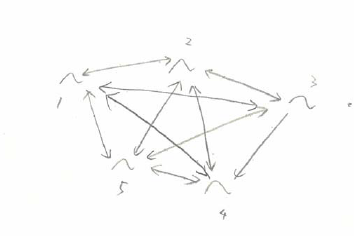
\includegraphics[width = 4.5cm]{1-3.png}
\end{wrapfigure}

As the simplest but likely the most relevant situation, suppose that any pair of two indistinguishable particles are interacting with each other in terms of ``two-body'' interaction potential

\begin{align}
\hat{V} \overset{def}{\equiv}\sum_{i<j}V^{(2)}({\bf x}_i,{\bf x}_j)
\end{align}

with

\[V^{(2)}({\bf x,y}) = V^{(2)}({\bf y,x}) \]

We assume that the interaction potential depends only on the spatial coordinates of two particles. 

\begin{align}
\begin{split}
\hat{V}|{\bf x}_1,\cdots,{\bf x}_n\rangle &= \sum_{i<j}V^{(2)}({\bf x}_i,{\bf x}_j)|{\bf x_1},\cdots,{\bf x}_n\rangle\\
&=\frac{1}{2}\sum_{i,j}V^{(2)}({\bf x}_i,{\bf x}_j)|{\bf x_1},\cdots,{\bf x}_n\rangle
\end{split}
\end{align}

Here is a multiparticle states for $5$ indistinguishable particles, which are located at ${\bf x}_1,{\bf x}_2,{\bf x}_3,{\bf x}_4,{\bf x}_5$, and represented by$|{\bf x}_1,{\bf x}_2,{\bf x}_3,{\bf x}_4,{\bf x}_5\rangle$

In terms of creation \& annihilation operators, this is given as follow

\begin{align}\label{eqs1.7.18}
V = \frac{1}{2}\int d^3{\bf x}\int d^3{\bf y}V^{(2)}({\bf x,y})a^\dagger({\bf x})a^\dagger({\bf y})a({\bf y})a({\bf x})
\end{align}

This can be verified by applying $V$ to $|{\bf x}_1,\cdots,{\bf x}_n\rangle$. 

\[\begin{split}
&a({\bf y})a({\bf x})|{\bf x}_1,\cdots,{\bf x}_n\rangle\\
&=a({\bf y})\sum_{k=1}^n\xi^{k-1}\delta^3({\bf x - x}_k)|{\bf x}_1,\cdots,{\bf x}_{k-1}{\bf x}_{k+1},\cdots,{\bf x}_n\rangle\\
&=\sum_{k=1}^n\xi^{k-1}\delta^3({\bf x-x}_k)\sum_{j=1,j\neq k}^n\eta_{jk}\delta^3({\bf y-x}_j)|{\bf x}_1,\cdots,(\text{no }{\bf x}_j\text{ and no }{\bf x}_k),\cdots,{\bf x}_n\rangle
\end{split}\]

where

\[\eta_{jk}=\begin{cases}
\xi^{j-1},\ \text{if }j<k\\
\ \\
\xi^{j-1},\ \text{if }j<k\\
\end{cases} \]

Then

\begin{align}
\begin{split}
&a^\dagger({\bf x})a^\dagger({\bf y})a({\bf y})a({\bf x})|{\bf x}_1,\cdots,{\bf x}_n\rangle\\
&=\sum_{j\neq k}\xi^{k-1}\eta_{jk}\delta^3({\bf x - x}_k)\delta^3({\bf y - x}_j)|\underset{{\bf x}_k}{\xout{\bf x}},\underset{{\bf x}_j}{\xout{\bf y}},{\bf x}_1,\cdots,(\text{no }{\bf x}_j,{\bf x}_k),\cdots,{\bf x}_n\rangle\\
&=\sum_{j\neq k}\delta^3({\bf x-x}_k)\delta^3({\bf y - x}_j)|{\bf x}_1,\cdots,{\bf x}_n\rangle
\end{split}
\end{align}

Multiplying by $\frac{1}{2}V^{(2)}(\bf x,y)$ and integrate over $\bf x$ and $\bf y$, we obtain this, so that this is correct. 

We might expect that the mutal interaction could also be described in terms of the particle density by

\begin{align}
V'=\frac{1}{2}\int d^3{\bf x}\int d^3{\bf y}V^{(2)}({\bf x,y})\hat{\rho}({\bf x})\hat{\rho}(\bf y)
\end{align}

with $\hat{\rho}({\bf x}) = a^\dagger({\bf x})a(\bf x)$

However, $V'$ is not quite the same as $V$ since 

\[\begin{split}
\rho({\bf x})\rho({\bf y}) &= a^\dagger({\bf x})a({\bf x})a^\dagger({\bf y})a({\bf y})\\
&=\xi a^\dagger({\bf x})a^\dagger({\bf y})a({\bf x})a({\bf y}) + \delta^3({\bf x-y})a^\dagger({\bf x})a({\bf y})\\
&= a^\dagger({\bf x})a^\dagger({\bf y})a({\bf y})a({\bf x}) + \delta^3({\bf x-y})a^\dagger({\bf x})a({\bf y})
\end{split}\]

so that

\[V' = V+\frac{1}{2}\int d^3{\bf x}V^{(2)}({\bf x,x})\hat{\rho}(\bf x) \]

Namely, $V'$ differs from $V$ by this extra term, which contributes to energy even when there is only one particle present. 

The true mutal interaction, which is $\hat{V}$, is zero unless there are two or more particles. 

We want only the mutal interaction, because this extra term can be included into the potential energy term appearing in the single-particle Hamiltonian. 

Moreover, for many physically relevant two-body interaction potentials, such as coulomb potential, $V'$ is infinite and is not what we would consider to be the true energy. 

\hrule

\ 

When we assume the two-body interaction potential depends only on spatial distance between two particles, 

\[V^{(2)}({\bf x,y}) = V({\bf x-y}) = V({\bf y-x}) \]

We can rewrite this mutual interaction part in terms of momentum representation

\begin{align}
\hat{V} = \frac{1}{2}\int\frac{d\bf q}{(2\pi)^3}\frac{d\bf p}{(2\pi)^3}\frac{d\bf p'}{(2\pi)^3}\tilde{V}({\bf q})a^\dagger({\bf p+q})a^\dagger({\bf p'-q})a({\bf p'})a({\bf p})
\end{align}

\begin{wrapfigure}{r}{5.5cm}
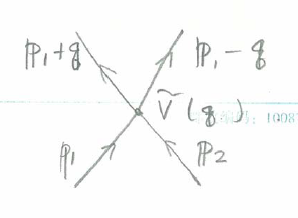
\includegraphics[width = 4.6cm]{1-4.png}
\end{wrapfigure}

where

\[\tilde{V}({\bf q})\equiv\int d^3{\bf x}V({\bf x})e^{_i\bf q\cdot x} \]

Note that this adds momentum $\bf q$ to one particle while substracts the same momentum $\bf q$ from the other with the amplitude of $\tilde{V}({\bf q})$

\begin{align}
\hat{V}|{\bf p}_1,{\bf p}_2\rangle = \frac{d\bf q}{(2\pi)^3}\tilde{V}({\bf q})|{\bf p}_1+{\bf q,p}_2-{\bf q}\rangle
\end{align}

This process is denoted by this diagram which is often called as Feynman diagram. 

\section{Degenerate electron gas}

So far, we have reviewed the $2$nd quantization. From the nextt weeks, we will study interacting fermi systems using $2$nd quantization Language. More specifically, we will often study a simple model that provides a first approximation to a metal. This system is an interacting electron gas placed in a uniformly distributed positive background. Because of the positive background, the total system is ensured to be neutral. In a real metal, the positive charge is localized in the ionic cores, whose dynamical motion must also be included in the calculation. 

However, these positive ions are usually much heavier than the electrons, so that it is permissible to neglect to ionic motions entirely. In contrast, the assumption of a uniform background is more drastic. In this sense, the present model can provide only a qualitative account of real metals in solids. 

We are interested in the properties of the bulk medium. Thus, it is convenient to enclose the system in a large cubic box with sides of length ``$L$''. The limit $L\rightarrow\infty$ will be taken at the end of the calculation. 

In a uniform infinite medium, all the physical properties must be invariant under spatial translation. This observation suggests the use of periodic boundary condition on the single-particle state;

\begin{align}
psi_{k,\lambda}({\bf x}) = \frac{1}{\sqrt{V}}e^{i\bf k\cdot x}\eta_{\lambda}
\end{align}

$V(\equiv L^3)$ is the volume of the box, $\eta_\lambda$ with $\lambda = \uparrow,\downarrow$ are the two spin functions for spin-up and spin-down

\begin{align}
\eta_\uparrow = \left(\begin{matrix}1\\0\end{matrix}\right),\eta_\downarrow = \left(\begin{matrix}0\\1\end{matrix}\right)
\end{align}

The periodic boundary condition determines the allowed wavelengths as

\begin{align}
{\bf k} = \frac{2\pi}{L}(n_x,n_y,n_z)
\end{align}

with $n_x,n_y,n_x = 0,\pm1,\pm2,\cdots,\pm\frac{L}{2}$. 

The total Hamiltonian of the system consists of three terms:

\begin{align}
H = H_el+H_b+H_{el-b}
\end{align}

where $H_{el}$ is the hamiltonian for the electrons:

\begin{align}
H_{el} = \sum_{i=1}^N\frac{P_i^2}{2m}+\frac{e^2}{2}\sum_{i\neq j}^N\frac{e^{-\mu|{\bf r}_i - {\bf r}_j|}}{|{\bf r}_i - {\bf r}_j|}
\end{align}

$H_b$ is the energy of the positive background whose particle density is $n(\bf x)$

\begin{align}
H_b = \frac{e^2}{2}\iint d^3{\bf x}d^3{\bf x'}\frac{n({\bf x})n({\bf x'})e^{-\mu|\bf x-x'|}}{|\bf x-x'|}
\end{align}

$H_{el-b}$ is the interaction energy between the electrons and the positively charged background

\begin{align}
H_{el-b} = -e^2\sum_{i=1}^N\int d^3{\bf x}\frac{n({\bf x})e^{-\mu|{\bf x-r}_i|}}{|{\bf x - r}_i|}
\end{align}

We have inserted an exponential convergence factor $\mu$ to define the integrals and this $\mu$ will be taken to be zero in the very end of the analysis. Because of the long-range nature of the coulomb interaction, these three terms ``individually'' diverge in the thermodynamics limit

($N\rightarrow\infty, V\rightarrow\infty$ with $n = N/V$ fixed)

However, the entire system is electrically neutral, so that the sum of these three terms must remains finite and meaningful in this limit. 

The convergence factor $\mu$ allows us to make this cancellation explicitly. 

Thus, our limiting procedure is firstly take the thermodynamic limit 

($N\rightarrow\infty, V\rightarrow\infty$ with $n = N/V$ fixed)

and then take $\mu\rightarrow0$. 

Equivalently, we can assume that $\mu^{-1}\ll L$ at each step of our following calculation. 

Now that the positive background $n(\bf x)$ is static, $H_b$ is a pure $c$-number, which can be easily evaluated for a uniform distribution of $n({\bf x})\equiv\frac{N}{V}$

\begin{align}
\begin{split}
H_b &=\frac{e^2}{2}\left(\frac{N}{V}\right)^2\iint d^3{\bf x}d^3{\bf x'}\frac{e^{-\mu|\bf x-x'|}}{|\bf x-x'|}\\
&=\frac{e^2}{2}\left(\frac{N}{V}\right)^2\int d^3{\bf x}\int d^3{\bf x}\frac{e^{-\mu|\bf z|}}{|\bf x|}
\end{split}
\end{align}%page99

Here we shifted the origin of the integration in the second line, which is allowed since $\mu^{-1}\ll L$. 

$N^{-1}\cdot H_b$ diverges in the limit of $\mu\to +0$, which represents the long-range nature of the coulomb interaction. 

$H_{el-b}$ is a one-particle operator for electron for static background $n({\bf x})$. 

For the uniform distribution, we may again use the translation invariant to estimate this as a $c$-number:

\begin{align}
\begin{split}
H_{el-b}&=-e^2\sum_{i=1}^N\frac{N}{V}\int d^3{\bf x}\frac{e^{-\mu|{\bf x-r}_i|}}{|{\bf x-r}_i|}\\
&=-e^2\sum_{i=1}^N\frac{N}{V}\int d^3{\bf x}\frac{e^{-\mu|{\bf x}}}{|{\bf x}|}\\
&=-e^2\frac{N^2}{V}\frac{4\pi}{\mu^2}
\end{split}
\end{align}

Thus the total Hamiltonian becomes 

\begin{align}\label{eq1.8.10}
\hat{H}=-\frac{e^2}{2}\frac{N^2}{V}\frac{4\pi}{\mu^2}+\hat{H}_{el}
\end{align}

so that all of the interacting physical effects are contained in $\hat{H}_{el}$. 

We now rewrite $H_{el}$ in terms of the $2$nd quantization language. We use a basis of momentum eigenstate with spin degree of freedom:

\[\psi_{{\bf k},\lambda}({\bf x})=\frac{1}{\sqrt{V}}e^{i\bf k\cdot x}\eta_\lambda \]

with $\lambda=\uparrow$ or $\downarrow$ \& ${\bf k}=\frac{2\pi}{L}(n_x,n_y,n_z)$

Correspongding creation \& annihilation operator has momentum \& spin indies, 

\[
\left.\begin{matrix}
a^\dagger_{{\bf k},\lambda} \\
\ \\
\underset{\text{momentum,spin}\quad}{a^\dagger_{{\bf k},{\lambda}}}
\end{matrix}\right\}\longrightarrow\psi_{{\bf k},\lambda}({\bf x})=\frac{1}{\sqrt{V}}e^{i\bf k\cdot x}\eta_\lambda 
\]

Moreover, the inner product between these `single-particle states' is given by

\[\begin{split}
\langle {\bf k},\lambda|{\bf k'},\lambda\rangle&\equiv\frac{1}{V}\int_V d^3{\bf x}\psi_{{\bf k},\lambda}^*({\bf x})\psi_{{\bf k'},\lambda'}({\bf x}) \\
&=\delta_{\lambda,\lambda'}\frac{1}{V}\int_V d^3{\bf x}e^{-i\bf (k-k')\cdot x}\\
&=\delta_{\lambda,\lambda'}\delta_{\bf k,k'}
\end{split}\]

with $\delta_{\bf k,k'}\equiv\delta_{n_x,n_x'}\delta_{n_y,n_y'}\delta_{n_z,n_z'}$

so that eq. \eqref{eqs1.6.5} tells that

\[[a_{{\bf k},\lambda},a^\dagger_{{\bf k'},\lambda}]\equiv\delta_{\lambda,\lambda'}\delta{\bf k,k'} \]

\dotfill

\ 

On the one hand, eq. \eqref{eqs1.7.6} suggests that the kinetic energy part is given by

\[\hat{T}\equiv\sum_{{\bf k}\lambda}\sum_{{\bf k'},\lambda'}a^\dagger_{{\bf k}\lambda} a_{{\bf k'},\lambda'}\langle{\bf k}\lambda|T|{\bf k'},\lambda'\rangle\]

where

\begin{align}\label{eq1.8.11}
\begin{split}
\langle{\bf k}\lambda|T|{\bf k'},\lambda'\rangle&\equiv\frac{\delta_{\lambda,\lambda'}}{V}\int d^3{\bf x}e^{-i\bf k\cdot x}\left(-\frac{\hbar^2\nabla^2}{2m}\right)e^{i\bf k'\cdot x}\\
&=\frac{\hbar^2 k^2}{2m}\delta_{\bf k,k'}\delta_{\lambda,\lambda'}\\
&\equiv\sum_{{\bf k},\lambda}\frac{\hbar^2\bf k^2}{2m}a^\dagger_{{\bf k}\lambda}a_{{\bf k}\lambda}
\end{split}
\end{align}

The two-particle interaction part can be evaluated from eq. \eqref{eqs1.7.18} as

\[\begin{split}
V=&\frac{e^2}{2}\int_V d^3{\bf x}\int_V d^3{\bf y}\sum_{\tau,\tau'}\frac{e^{-\mu|\bf x-y|}}{|\bf x-y|}\left( \sum_{{\bf k}_1,\lambda_1}\psi^*_{{\bf k}_1,\lambda_1}({\bf x},\tau)a_{{\bf k}_1,\lambda_1}^\dagger\right)\times\left( \sum_{{\bf k}_2,\lambda_2}\psi^*_{{\bf k}_2,\lambda_2}({\bf y},\tau')a_{{\bf k}_2,\lambda_2}^\dagger\right)\\
&\times\left( \sum_{{\bf k}_4,\lambda_4}a_{{\bf k}_4,\lambda_4}\psi_{{\bf k}_4,\lambda_4}({\bf y},\tau')\right)\times\left( \sum_{{\bf k}_3,\lambda_3}a_{{\bf k}_3,\lambda_3}\psi_{{\bf k}_3,\lambda_3}({\bf x},\tau)\right)
\end{split}\]

Since we consider a spinful fermion here, 

\[\int d^3{\bf x}\int d^3{\bf y}a^\dagger({\bf x})a^\dagger({\bf y})a({\bf y})a({\bf x})V^{(2)}({\bf x,y})\to\sum_\tau \sum_{\tau'}\int d^3{\bf x},\tau)a^\dagger({\bf y},\tau')a({\bf y},\tau')a({\bf x},\tau)\times V^{(2)}(\bf x,y)\]

We changed the single particle basis from coordinate to momentum

\[\begin{cases}
a^\dagger({\bf x},\tau)&=\sum_{{\bf k}\lambda}\psi_{{\bf k},\lambda}^*({\bf x},\tau)a^\dagger_{{\bf k},\lambda}\\
\ & \\
a({\bf x},\tau)&=\sum_{{\bf k'}\lambda'}\psi_{{\bf k'},\lambda'}({\bf x},\tau)a_{{\bf k'},\lambda'}
\end{cases}\]

\[V=\frac{1}{2}\sum_{{\bf k}_1,\sim,{\bf k}_4}\sum_{\lambda_1,\sim,\lambda_4}\langle{\bf k}_1,\lambda_1,{\bf k}_2,\lambda_2|V|{\bf k}_4,\lambda_4,{\bf k}_3,\lambda_3\rangle\times a^\dagger_{{\bf k}_1,\lambda_1}a^\dagger_{{\bf k}_2,\lambda_2}a_{{\bf k}_4,\lambda_4}a_{{\bf k}_3,\lambda_3}\]

where

\[\begin{split}
\langle{\bf k}_1,\lambda_1,{\bf k}_2,\lambda_2|V|{\bf k}_4,\lambda_4,{\bf k}_3,\lambda_3\rangle &=\frac{e^2}{V}\iint d^3{\bf x}d^3{\bf y}\sum_{\tau}\sum_{\tau'}e^{-i{\bf k}_1\cdot\bf x}\eta_{\lambda_1}^\dagger(\tau)e^{_i{\bf k}_2\cdot\bf y}\eta_{\lambda_2}^\dagger(\tau')\frac{e^{-\mu|\bf x-y|}}{|\bf x-y|}e^{-{\bf k}_4\cdot\bf y}\eta_{\lambda_4}(\tau')e^{i{\bf k}_3\cdot\bf x}\eta_{\lambda_3}(\tau)\\
&=\frac{e^2}{V^2}\int d^3{\bf y}e^{-i({\bf k}_1 + {\bf k}_2 - {\bf k}_3 - {\bf k}_4)\cdot\bf y}\times\int d^3{\bf x}e^{i({\bf k}_3-{\bf k}_1)\cdot\bf x}\frac{e^{-\mu|\bf x|}}{|\bf x|}\delta_{\lambda_1,\lambda_3}\delta_{\lambda_2,\lambda_4}\\
&=\frac{e^2}{V}\delta_{\lambda_1,\lambda_3}\delta_{\lambda_2,\lambda_4}\delta_{{\bf k}_1 + {\bf k}_2,{\bf k}_3 + {\bf k}_4}\times\frac{4\pi}{({\bf k}_1 - {\bf k}_3)^2+\mu^2}
\end{split}\]

Thus, with ${\bf k}_1 - {\bf k}_3 = \bf q$, we have

\begin{align}
\hat{V}=\frac{e^2}{2V}\sum_{\bf k,p,q}\sum_{\lambda_1,\lambda_2}\frac{4\pi}{{\bf q^2}+\mu^2}a^\dagger_{{\bf k+q},\lambda_1}a^\dagger_{{\bf p-q},\lambda_2}a_{{\bf p},\lambda_2}a_{{\bf k},\lambda_1}
\end{align}

It is convenient to separate the summation over $\bf q$ into two parts

\begin{align}\label{eq1.8.13}
V=\frac{e^2}{2V}\sum_{\bf k,p}\sum_{{\bf q}\neq0}\sum_{\lambda_1,\lambda_2}\frac{4\pi}{{\bf q^2}+\mu^2}a^\dagger_{{\bf k+q},\lambda_1}a^\dagger_{{\bf p-q},\lambda_2}a_{{\bf p},\lambda_2}a_{{\bf k},\lambda_1} + \frac{e^2}{2V}\sum_{\bf k,p}\sum_{\lambda_1,\lambda_2}\frac{4\pi}{\mu^2}a^\dagger_{{\bf k},\lambda_1}a^\dagger_{{\bf p},\lambda_2}a_{{\bf p},\lambda_2}a_{{\bf k},\lambda_1}
\end{align}

where the first term refers to $\bf q\neq0$ while the second term refers to $\bf q=0$. The second term can be further evaluated as 

\[\text{second term}= \frac{e^2}{2V}\sum_{\bf k,p}\sum_{\lambda_1,\lambda_2}\frac{4\pi}{\mu^2}a^\dagger_{{\bf k},\lambda_1}a_{{\bf k},\lambda_1}(a^\dagger_{{\bf p},\lambda_2}a_{{\bf p},\lambda_2}-\delta_{\bf k,p}\delta_{\lambda_1,\lambda_2}) = \frac{e^2}{2V}\frac{4\pi}{\mu^2}(\hat{N}^2-\hat{V})\]

where $\hat{N}\equiv\sum_{{\bf k}\lambda}a_{{\bf k},\lambda}^\dagger a_{{\bf k},\lambda}$ is an operator representing the total number of electrons (see eq. \eqref{eqs1.7.15} also). 

In a sub-Hilbert space of fixed number of electrons, we can replace this by a $c$-number $N$ so that the $2$nd term reduces to a $c$-number

\[\text{second term}=\frac{e^2}{2}\frac{N^2}{V}\frac{4\pi}{\mu^2}-\frac{e^2}{2}\frac{N}{V}\frac{4\pi}{\mu^2}\]

putting this into eq. \eqref{1.8.13} abd substituting eqs. \eqref{eq1.8.13} \& \eqref{eq1.8.11} into eq. \eqref{eq1.8.10}, we finally have

\[\hat{H}=-\frac{e^2}{2}\frac{N^2}{V}\frac{4\pi}{\mu^2}+\sum_{{\bf k},\lambda}\frac{\hbar^2\bf k^2}{2m}a^\dagger_{{\bf k},\lambda}a_{{\bf k},\lambda}+\frac{e^2}{2V}\sum_{\bf k,p} \sum_{{\bf q}\neq0}\sum_{\lambda_1,\lambda_2}\frac{4\pi}{{\bf q^2}+\mu^2}a^\dagger_{{\bf k+q},\lambda_1}a^\dagger_{{\bf p-q},\lambda_2}a_{{\bf p},\lambda_2}a_{{\bf k},\lambda_1} + \frac{e^2}{2}\frac{N^2}{V}\frac{4\pi}{\mu^2}-\frac{e^2}{2}\frac{N}{V}\frac{4\pi}{\mu^2} \]

The last term represents an energy per particlem $-\displaystyle\frac{e^2}{2}\frac{4\pi}{V\mu^2}$, which vanished in the thermodynamic limit with $\mu^{-1}\ll L$. 

Therefore, it is now clear that these two terms, each of which diverges in the limit of $\mu\to0$ respectively, cancel each other, so that the entire Hamiltonian has no trivially diverging term. This comes from the electric neutrality of the entire system. 

Furthermore, it is now permissible to set $\mu=0$ here, because this summation excludes $\bf q=0$ and the summand is always well defined even at $\mu =0$. 

We thus reach the final Hamiltonian for a bulk electron gas in a uniformly distributed positively-charged background. 

\begin{align}\label{eq1.8.14}
\hat{H}=\sum_{{\bf k},\lambda}\frac{\hbar^2\bf k^2}{2m}a^\dagger_{{\bf k},\lambda}a_{{\bf k},\lambda} + \frac{e^2}{2V}\sum_{\bf k,p} \sum_{{\bf q}\neq0}\sum_{\lambda_1,\lambda_2}\frac{4\pi}{{\bf q^2}}a^\dagger_{{\bf k+q},\lambda_1}a^\dagger_{{\bf p-q},\lambda_2}a_{{\bf p},\lambda_2}a_{{\bf k},\lambda_1}
\end{align}

where the limit $N\to\infty, V\to\infty$ with $N/V=n=$constant is implicitly assumed. 

We often call this model as a model of degenerate electron gas or a model for Fermi gas with long-range Coulomb interaction. This model is a prototype model for studying the physical properties of a metal in solids. 

\dotfill

\ 

From the next class, I will go to $\cdots$ general theory framework for many-body systems, especially focusing on interacting fermion systems. 